\documentclass[10pt,a4paper]{article}

\usepackage[left=2.2cm, right=2.2cm, top=2cm, bottom=2.2cm, footskip=0.9cm]{geometry}
\usepackage{amsmath}
\usepackage{fontspec}
\usepackage{unicode-math}
\usepackage{graphicx}
\usepackage{array}
\usepackage{booktabs}
\usepackage{colortbl}
\usepackage{xcolor}
\usepackage{caption}
\usepackage[section]{placeins}
\usepackage{titlesec}
\usepackage{enumitem}
\usepackage{ragged2e}
\usepackage{fancyhdr}
\usepackage{microtype}
\usepackage[colorlinks, urlcolor=accent, linkcolor=ink]{hyperref}

%% ---------------------------------------------------------------- type
%% TeX Gyre Termes (a free Times New Roman clone) ships in fonts/, so the charts and the document match
\setmainfont{texgyretermes}[Path=fonts/, Extension=.otf, UprightFont=*-regular, ItalicFont=*-italic,
  BoldFont=*-bold, BoldItalicFont=*-bolditalic]
\newfontfamily\headfont{texgyretermes}[Path=fonts/, Extension=.otf, UprightFont=*-bold]
\newfontfamily\capsfont{texgyretermes}[Path=fonts/, Extension=.otf, UprightFont=*-bold, LetterSpace=10]
\setmathfont{texgyretermes-math.otf}
\setmonofont{texgyrecursor}[Extension=.otf, UprightFont=*-regular]

%% ---------------------------------------------------------------- colour
\definecolor{ink}{HTML}{111827}
\definecolor{body}{HTML}{1F2937}
\definecolor{muted}{HTML}{6B7280}
\definecolor{rule}{HTML}{D1D5DB}
\definecolor{accent}{HTML}{004225}
\color{body}
\arrayrulecolor{rule}

%% ---------------------------------------------------------------- layout
\renewcommand{\normalsize}{\fontsize{10}{13}\selectfont}
\normalsize
\setlength{\parindent}{0pt}
\setlength{\parskip}{4pt}
\setlength{\textfloatsep}{12pt plus 2pt}
\setlength{\intextsep}{10pt plus 2pt}
\RaggedRight
\graphicspath{{figures/}}

\renewcommand{\thesection}{0\arabic{section}}
\titleformat{\section}{\headfont\fontsize{14.5}{17}\selectfont\color{ink}}
  {{\color{accent}\thesection}}{0.6em}{}
\titlespacing*{\section}{0pt}{12pt plus 2pt}{2pt}

\DeclareCaptionFont{muted}{\color{muted}}
\DeclareCaptionFont{ink}{\color{ink}}
\captionsetup{font={small,muted}, labelfont={bf,ink}, labelsep=period,
  justification=centering, singlelinecheck=false, skip=4pt}

\pagestyle{fancy}
\fancyhf{}
\renewcommand{\headrulewidth}{0pt}
\fancyfoot[L]{\small\color{muted}Padraig Middleton\enspace·\enspace Pricing options with the Fourier transform}
\fancyfoot[R]{\small\color{muted}\thepage}

\setlist[itemize]{leftmargin=11pt, itemsep=1.5pt, topsep=3pt, parsep=0pt,
  label={\color{accent}\textbullet}}
\setlength{\abovedisplayskip}{6pt}
\setlength{\belowdisplayskip}{6pt}

\newcommand{\vol}{\mathrm{vol}}

%% the one-line plain-English summary under each heading
\newcommand{\lead}[1]{{\itshape\fontsize{11}{14}\selectfont\color{accent}#1}\par\vspace{1pt}}

%% headline numbers
\newcommand{\statnum}[1]{{\headfont\fontsize{21}{24}\selectfont\color{ink}#1}}
\newcommand{\statlabel}[1]{{\small\color{muted}#1}}

\begin{document}

%% ---------------------------------------------------------------- header
{\capsfont\fontsize{7.5}{9}\selectfont\color{accent}OPTION PRICING\enspace·\enspace PYTHON PROJECT}\par
\vspace{6pt}
{\headfont\fontsize{25}{29}\selectfont\color{ink}Pricing options with the Fourier transform}\par
\vspace{4pt}
{\itshape\fontsize{14}{17}\selectfont\color{muted}Every strike at once, from the model's fingerprint}\par
\vspace{6pt}
{\small\color{muted}Padraig Middleton\enspace·\enspace October 2026\enspace·\enspace
\href{https://github.com/poggey/fourier-option-pricing}{github.com/poggey/fourier-option-pricing}}\par
\vspace{11pt}

\noindent
\begin{tabular}{@{}>{\RaggedRight}p{0.28\linewidth}|@{\hspace{14pt}}>{\RaggedRight}p{0.28\linewidth}|@{\hspace{14pt}}>{\RaggedRight}p{0.32\linewidth}@{}}
\statnum{4,096} & \statnum{0.2 ms} & \statnum{6 × 10\smash{\textsuperscript{−14}}} \\[2pt]
\statlabel{strikes priced in one FFT pass} &
\statlabel{for every strike, over 9,000× faster than one at a time} &
\statlabel{largest gap from Black-Scholes}
\end{tabular}

\vspace{8pt}
I built an option pricer that only needs a model's \emph{fingerprint} (the Fourier transform of where
the share might end up), then checked it against Black-Scholes, where the right answer is known.

\begin{center}
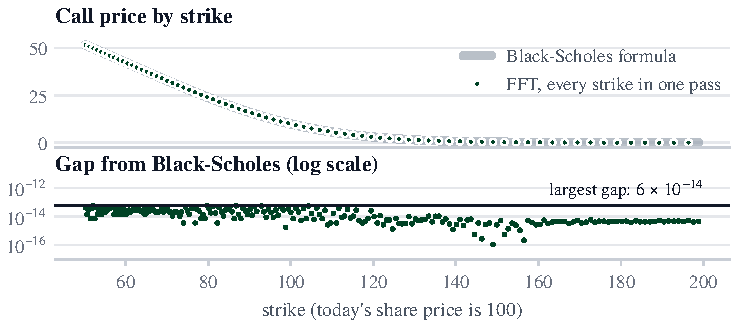
\includegraphics{fft_accuracy.pdf}
\captionof{figure}{One FFT pass against the Black-Scholes formula, at the 225 grid strikes from 50 to 200.}
\label{fig:accuracy}
\end{center}

%% ---------------------------------------------------------------- 1
\section{The idea}

\lead{An option's price is an average over everywhere the share could end up.}

\begin{itemize}
\item For realistic models those chances have no formula, but their fingerprint usually does.
\item So I price options from the fingerprint alone (Carr and Madan, 1999), with the FFT doing every strike at once.
\item Why it matters: banks re-price thousands of options every time they fit a model to market prices.
\end{itemize}

%% ---------------------------------------------------------------- 2
\section{Notation}

\lead{Everything is measured in logs, because shares move in percentages.}

\begin{itemize}
\item A 10\% rise and a 10\% fall become equal steps, so the outcomes form a symmetric bell curve.
\item Running example: share at 100, strike 100, one year, 4\% interest, 20\% volatility.
Its exact Black-Scholes price is 9.925054.
\end{itemize}

\vspace{2pt}
{\centering\footnotesize\renewcommand{\arraystretch}{0.98}
\begin{tabular}{@{}llll@{}}
\toprule
\color{muted}Symbol & \color{muted}Plain name & \color{muted}The idea & \color{muted}Example \\
\midrule
$S_0$ & Today's share price & Where the share starts & 100 \\
$K$ & Strike & The fixed price you can buy at & 100 \\
$T$, $r$ & Time, interest rate & Years until the option ends; what money earns meanwhile & 1, 4\% \\
$\vol$ & Volatility & How much the share typically moves in a year & 20\% \\
$s$, $k$ & Log final price, log strike & The final price and the strike on the percentage scale & $k = \ln 100 = 4.605$ \\
$q(s)$ & Probability curve & How likely each log final price is & a bell curve \\
$C(k)$, $D(k)$ & Call price, damped price & What the option is worth at each strike; the same, damped & 9.925 \\
$a$ & Damping strength & How hard the left end of the price curve is pushed down & 1.5 \\
$u$, $v$ & Spin speeds & How fast the arrows turn: $u$ for chances, $v$ for prices & \\
$F(u)$, $W(v)$ & Fingerprint, wound-up price & The average arrow; the damped price in frequency world & \\
\bottomrule
\end{tabular}\par}
\vspace{2pt}

%% ---------------------------------------------------------------- 3
\section{The price is an average}

\lead{Fair price = average payoff, weighted by how likely each outcome is, then discounted.}

\begin{itemize}
\item A call pays $\max(S_T - K,\,0)$: with strike 100, ending at 120 pays 20 and ending at 90 pays nothing.
\item Toy version: the share ends at 80, 100 or 120 (25\%, 50\%, 25\%). Only 120 pays (20), so the
price is $0.25 \times 20 \times e^{-0.04} \approx 4.80$.
\item Real version: the outcomes become a curve and the sum becomes an integral.
\end{itemize}
\[ C(k) = e^{-rT}\int_{k}^{\infty}\left(e^{s} - e^{k}\right) q(s)\,ds \]
\begin{itemize}
\item Under Black-Scholes, $q$ is a bell curve with centre $m = \ln S_0 + (r - \tfrac12\vol^2)T = 4.6252$
and spread $\vol\sqrt{T} = 0.20$.
\item The height is chance \emph{per unit width}: 2.0 at the centre means about a 2\% chance of ending within 1\%.
\end{itemize}

\begin{figure}[!htb]
\centering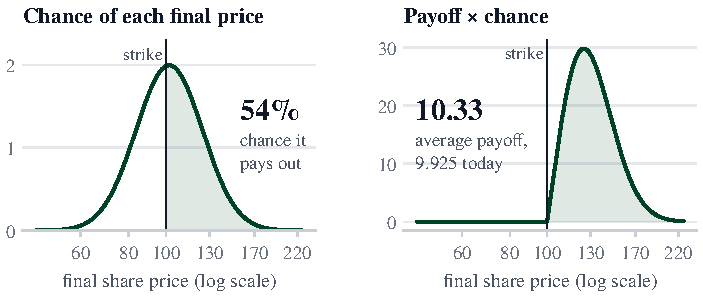
\includegraphics{price_as_average.pdf}
\caption{Shaded on the left: the chance it pays out, 54\% ($N(d_2)$ in Black-Scholes). On the right: the
average payoff, 10.33.}
\label{fig:average}
\end{figure}

%% ---------------------------------------------------------------- 4
\section{The fingerprint}

\lead{Turn every outcome into an arrow, weight it by its chance, and average. That's the fingerprint.}

\begin{itemize}
\item $e^{ix} = \cos x + i\sin x$ is an arrow of length 1 at angle $x$. At spin speed $u$, outcome $s$
points at angle $us$.
\item Writing each outcome as centre plus deviation, $s = m + x$, the average splits into two parts:
\end{itemize}
\[ F(u) = \int e^{ius}\, q(s)\, ds
   = \underbrace{e^{ium}}_{\text{rotation}} \times \underbrace{e^{-\frac{1}{2}\vol^2 T u^2}}_{\text{shrink}} \]
\begin{itemize}
\item Rotation: where the outcomes are. Shrink: how spread out they are, as the arrows fan out and cancel.
\item The payoff isn't in it, so a new model means changing only this one function.
\end{itemize}

\begin{figure}[!htb]
\centering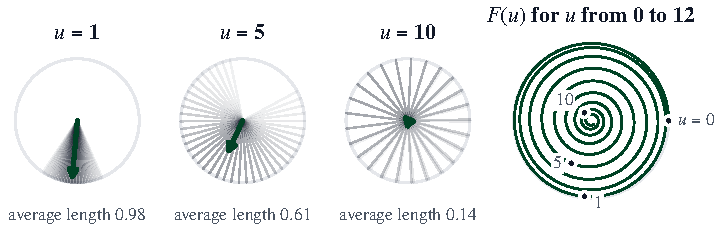
\includegraphics{fingerprint.pdf}
\caption{Grey: each outcome's arrow. Green: their average, which shrinks and spirals in as the spin speeds up.}
\label{fig:fingerprint}
\end{figure}

\begin{figure}[!htb]
\noindent\begin{minipage}[c]{0.36\linewidth}
\textbf{The plan.} I only know the share through its fingerprint, which lives in frequency world. So I move
the call price there, work it out, and bring it back in four steps.
\end{minipage}\hfill
\begin{minipage}[c]{0.6\linewidth}
\centering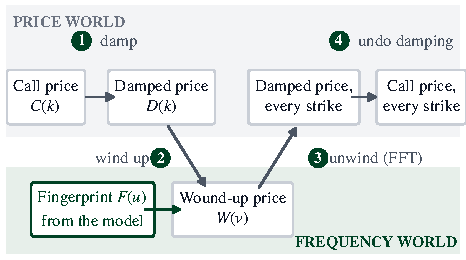
\includegraphics{round_trip.pdf}
\captionof{figure}{Step 2 never needs any prices: it's built from the fingerprint.}
\label{fig:roundtrip}
\end{minipage}
\end{figure}

%% ---------------------------------------------------------------- 5
\section{The snag: damping}

\lead{The call price never dies away on the left, so I push it down before transforming it.}

\begin{itemize}
\item Right end: the price falls to zero, since the share would have to double to pass strike 200.
\item Left end: buying the share for almost nothing is worth about 100, however small the strike.
\item Fix: multiply by $K^a$, which is tiny on the left. Strike 0.0001 goes from 99.9999 to 0.0001.
\end{itemize}
\[ D(k) = e^{ak}\, C(k) = K^{a} \times C \]
\begin{itemize}
\item Nothing is lost: multiplying by $e^{-ak}$ at the end undoes it.
\end{itemize}

\begin{figure}[!htb]
\centering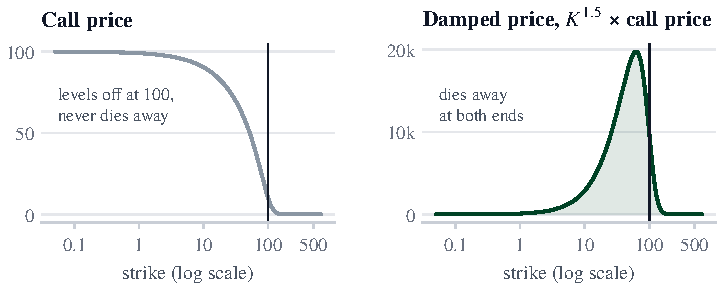
\includegraphics{damping.pdf}
\caption{Left: levels off at 100. Right: damped by $K^{1.5}$, it dies away at both ends.}
\label{fig:damping}
\end{figure}

%% ---------------------------------------------------------------- 6
\section{Winding it up}

\lead{Swap the order: wind up each outcome across strikes, then average. That needs only the payoff and the fingerprint.}

A small version first: 3 outcomes, 3 strikes, damping 1.5. Each cell is chance $\times\, K^{1.5} \times$ payoff.

\begin{center}\footnotesize
\begin{tabular}{@{}lrrrr@{}}
\toprule
\color{muted}Strike / outcome & \color{muted}80 (25\%) & \color{muted}100 (50\%) & \color{muted}120 (25\%) & \color{muted}Row total \\
\midrule
70  & 1,464 & 8,785 & 7,321 & \textbf{17,570} \\
90  & 0     & 4,269 & 6,404 & \textbf{10,673} \\
110 & 0     & 0     & 2,884 & \textbf{2,884} \\
\midrule
Column total & \textbf{1,464} & \textbf{13,054} & \textbf{16,609} & 31,127 \\
\bottomrule
\end{tabular}
\end{center}

\begin{itemize}
\item \textbf{Rows} add up to damped prices. That needs the price at every strike, which I don't have.
\item \textbf{Columns} add up to one outcome's share. That needs only the payoff and its chance.
\item Same grand total either way: $-23{,}141 + 18{,}532i$ here at $v = 2$, and 30,520.88 for the full curve.
\item Each column has a closed form, so the whole table collapses to one formula:
\end{itemize}
\[ W(v) = \frac{e^{-rT}\, F\big(v - (a+1)i\big)}{a^2 + a - v^2 + i(2a+1)v} \]
\begin{itemize}
\item Discounting, times the chances (fingerprint at a shifted speed), over the payoff's shape. Damping must be
positive, or the bottom hits zero at $v = 0$.
\end{itemize}

\begin{figure}[!htb]
\centering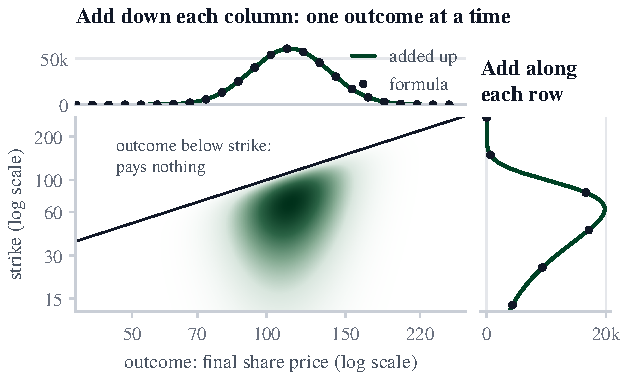
\includegraphics{table.pdf}
\caption{The full table at $v = 0$. Columns match the formula, rows match the damped prices; both total 30,520.88.}
\label{fig:table}
\end{figure}

%% ---------------------------------------------------------------- 7
\section{Unwinding with the FFT}

\lead{Unwind back to strikes and undo the damping. The FFT does every strike at once.}

\[ C(k) = \frac{e^{-ak}}{\pi}\int_0^{\infty}\text{Re}\left[e^{-ivk}\, W(v)\right] dv \]
\begin{itemize}
\item Why $\frac{1}{\pi}$: the full unwind has $\frac{1}{2\pi}$, but prices are real, so $+v$ and $-v$ pair
up and only half is needed.
\item Strike 100: the integral is about 31,180, and $31{,}180 / (100^{1.5}\pi) = 9.925$.
\item If (gap between spin speeds) $\times$ (gap between log strikes) $= 2\pi/N$, the sum is exactly an FFT.
\item For 4,096 strikes that's about 49,000 steps instead of 16.8 million, with strikes 0.6\% apart.
\end{itemize}

%% ---------------------------------------------------------------- 8
\section{Results}

\lead{It matches Black-Scholes to 12 decimal places, over 9,000 times faster than one strike at a time.}

\begin{itemize}
\item Accuracy: largest gap $6\times10^{-14}$ across the 225 strikes from 50 to 200 (Figure~\ref{fig:accuracy}).
\item Single strikes: 23.906164, 9.925054 and 2.999949 at strikes 80, 100 and 120. Damping 1.0 gives the same.
\item Speed, on my laptop: 0.2 ms for all 4,096 strikes by FFT, against 0.5 ms \emph{per strike} one at a time.
\end{itemize}

%% ---------------------------------------------------------------- 9
\section{Limits and next steps}

\lead{Two settings decide how accurate it is. Next, I want a model where shares can crash.}

\begin{itemize}
\item Damping: the gap is $6\times10^{-14}$ at 1.5, but $1\times10^{-9}$ at 1.0 and $4\times10^{-4}$ at 0.5.
\item Grid: spin speeds 1.0 apart put strikes 0.15\% apart, but the gap grows to $8\times10^{-3}$.
\item European options only: one payoff, on one fixed date.
\item \textbf{Next:} a jump model (Merton's) needs only a new fingerprint, and should show why crash insurance
has cost more than Black-Scholes says since 1987. Then fit it to real market prices.
\end{itemize}

\end{document}
